\section{Fabuła w grach RTS (Bogna Lew)}\label{s:fabula}
W przypadku wielu gier, niezależnie od gatunku, kluczową rolę odgrywa fabuła. To ona sprawia, że gra przestaje być
jedynie programem wykonującym polecenia, a staje się opowieścią będącą formą rozrywki. Ważnym aspektem fabuły jest jej
narracja, która definiuje kolejność występowania konkretnych elementów. W odróżnieniu od narracji budującej
fabułę książki, czy filmu, narracja w grach komputerowych umożliwia graczowi wpływanie na nią. "Dobrze nakreślona
narracja wykorzystuje wybory fabularne z wielkim uwzględnieniem ogólnego celu pracy. Może obejmować ujawnienie pewnych
informacji z przeszłości, aby zwiększyć poczucie niepewności, lub wczesne informacje podstawowe, aby wzmocnić motywację
postaci" \cite{level_design}.

W grach komputerowych w skład fabuły wchodzą cel główny oraz zadania poboczne. Cel główny stanowi podstawę gry, dając
graczowi poczucie dążenia do czegoś i jest ogólnym zamysłem całej rozgrywki. Zadania poboczne natomiast są krótkimi
misjami będącymi urozmaiceniem rozgrywki. "W odniesieniu do gier komputerowych można więc mówić o podwójnym motywowaniu
ich użytkowników, które dokonuje się na dwóch narracyjnych poziomach: jedna z motywacji wyznacza cel całej
rozgrywce, druga natomiast jest ulokowana w przestrzeni pojedynczej misji i kończy wraz z jej zakończeniem" \cite{olbrzymwcieniu}.

Innym elementem budującym fabułę są przerywniki filmowe, które wprowadzają nowe informacje i wydarzenia. "Wiele gier z
wyrafinowaną fabułą wykorzystuje tę technikę do umiejscowienia działań gracza w fikcyjnym świecie, który dzięki temu
może zostać opisany z dużą kontrolą po stronie autora" \cite{understanding_games}. Stanowią one ciekawe urozmaicenie w rozgrywce i
pozwalają na przekazanie graczowi więcej informacji.

W przypadku gier strategii czasu rzeczywistego fabuła występuje w trybie kampanii tych gier. Każda z pojedynczych bitew
stanowi fragment większej historii występującej w kampanii. Typowo w grach typu RTS występuje fabuła liniowa.
Przykładowo w grze \textit{Warhammer 40,000: Dawn of War} ogólnym zamysłem kampanii jest obrona planety przed najazdem wroga.
Zrealizowana jest za pomocną jedenastu misji, w których gracz ma do realizacji pewne cele, takie jak zajęcie określonej
liczby punktów kontrolnych, czy zniszczenie bazy przeciwnika. Pomiędzy misjami występują przerywniki filmowe, które
to odkrywają przed graczem kolejne elementy historii.

W tym miejscu warto wspomnieć System Nemesis występujący w grze \textit{Middle-earth: Shadow of Mordor} i rozwinięty w
\textit{Middle-earth: Shadow of War}\footnote{\url{https://www.shadowofwar.com/}}. Chociaż wymienione gry nie są z gatunku strategii czasu rzeczywistego to ta mechanika jest
interesującym przykładem kształtowania fabuły w grze. System Nemesis jest mechanizmem generowania przeciwników, który nadaje
każdemu z nich ich unikalny charakter oraz wygląd. W ciągu gry system Nemesis dynamicznie wpływa na postacie, rozwijając
je i odpowiednio zmieniając ich wygląd. Efektem tego jest płynnie zmieniająca się fabuła, która dla każdego gracza
będzie inna.

Do podstawowych elementów tej mechaniki należy rozbudowany system relacji pomiędzy postaciami w grze, w tym postaci
gracza. Dodatkowo buduje ona hierarchię wśród Orków, dynamicznie ją aktualizując w trakcie gry w zależności od śmierci
poszczególnych bohaterów oraz postaci gracza.

\begin{figure}[h!]
    \centering
    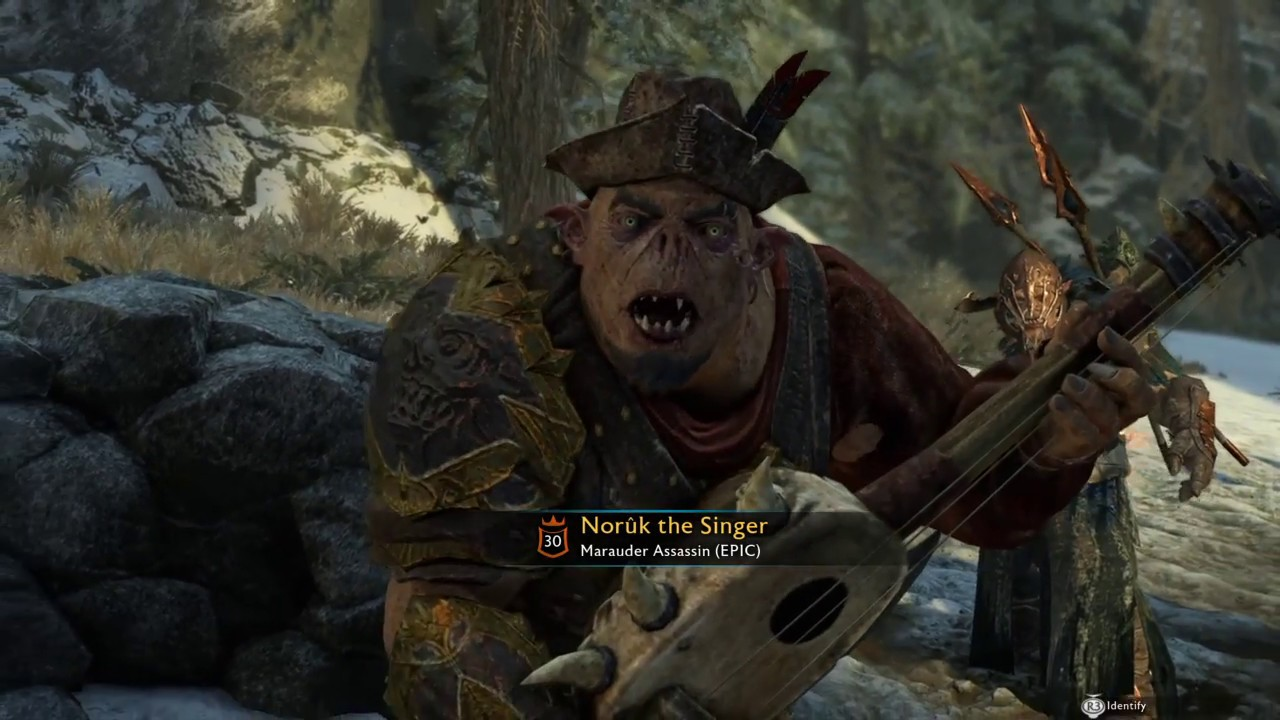
\includegraphics[width=0.9\textwidth]{images/system_nemesis.jpg}
    \caption{Przykładowa postać przeciwnika utworzona przez system Nemesis.}
\end{figure}

System Nemesis jest interesującą mechaniką budującą fabułę w grze. Pozwala na zbudowanie unikatowych przeciwników,
którzy mają bezpośredni wpływ na rozgrywkę i kształtowanie jej przebiegu.